\section{Transformers}
\begin{figure}[h]
\centering
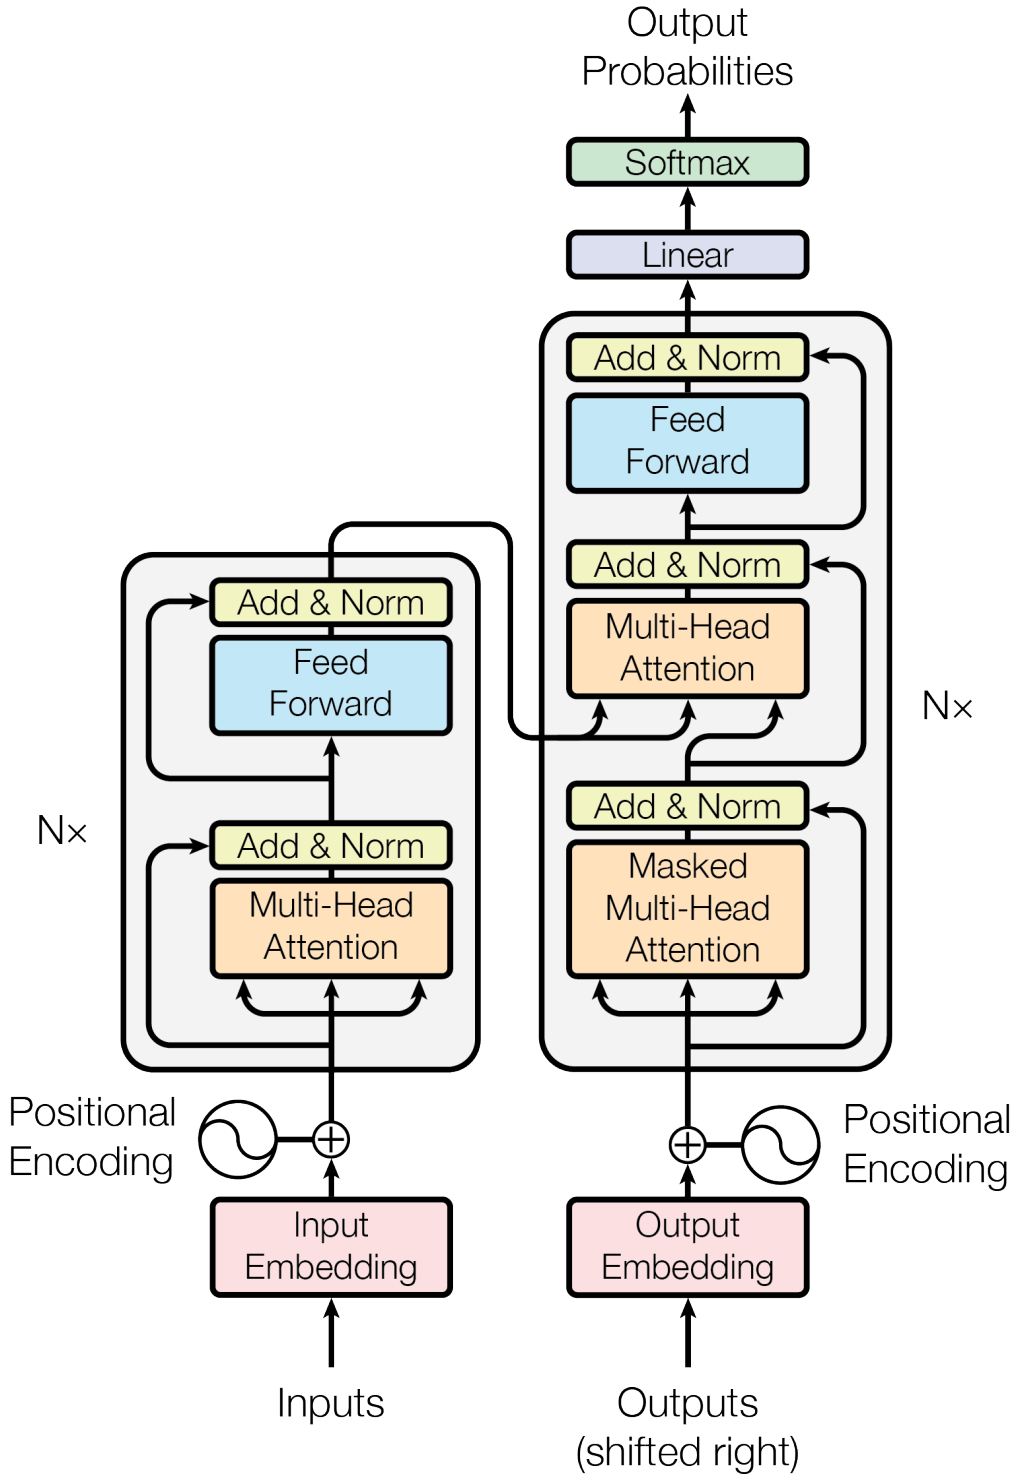
\includegraphics[width=0.5\textwidth]{Transformer model diagram}
\caption{Diagram depicting the architecture of the transformer model from \citet{AttentionIsAllYouNeed}.}
\end{figure}
\subsection{Problems solved by transformers}
The point of transformers was to overcome the problems faced by the previous state-of-the-art architectures while still including prominent aspects of the RNN and Convolutional Neural Network (CNN) models.

The RNN model has two notable weaknesses. First is its inability to learn long-term patterns, due to the exploding and vanishing gradient problems that occur during backpropagation.
Secondly, its recurrent connection is also a weakness. This is because it is not possible to compute the cell at time step $i$ until the cell at time step $i-1$ has been computed as information is propagated along a sequence.

In contrast, one of the benefits of CNNs is that they can be computed concurrently. However, unlike RNNs, they are unable to learn even short-term patterns. The size of the patterns they can learn is limited by their architecture.

Transformers attempt to feature the best of both techniques.
Transformers can model dependencies over the whole range of the input sequence as easily they can model neighboring sequences. And there are no recurrent connections, allowing efficient computation using parallelization. This is facilitated through the use of the self-attention mechanism.\cite{TransformersScratchPeterbloem}


\subsection{Self-attention Mechanism}

- snak om time embedding 
- måske snak om convoluted neural networks 
- afslut med at gennemgå den overordnede struktur, vi bruger i vores model - (similar to BERT)

With self-attention, the model can learn to associate different input.
To achieve this, three input vectors are needed - queries and keys of dimension $d_k$, and values of dimension $d_v$.
The attention function maps the query and the set of key-value pairs to some output, where the output is a weighted sum of the values.
The weight of each value is calculated using a compatibility function.
This weight denotes how compatible the query is with the given key.



The output matrix of weights is computed using the function
$$
Attention(Q, K, V) = softmax(\frac{QK^T}{\sqrt{d_k}})V
$$

Additive attention and dot product attention are among some of the most common attention functions used.
For the purposes of this project, we decided to use the scaled dot product attention technique with the scaling factor $\frac{1}{\sqrt{d_k}}$.
We use this technique as it is faster and more space-efficient as argued in \citet{AttentionIsAllYouNeed}.

Because the dot product can result in values between negative and positive infinity, the \textit{softmax} activation function is used to map values to the interval $[0,1]$, and to ensure that they sum to $1$ over the entire sequence.

\subsection{Multi-Head Attention}
To improve the self-attention mechanism, the authors of the original transformer model implemented multi-head attention.
This is a module that runs through the previously described attention mechanism multiple times and in parallel.
It then concatenates the attention weights of all the independent self-attention layers. 

\begin{align*}
MultiHead(Q, K, V) = Concat(h_1, \ldots, h_i)W^O \\
\text{where }h_i = Attention(QW^Q_i, KW^K_i, VW^V_i) 
\end{align*}

In the model we use, the weights are then passed through a dense layer in which a non-linear transformation is applied using the \textit{ReLU} activation function rather than a linear transformation as described in \citet{AttentionIsAllYouNeed}.


\subsection{How transformers work}
Transformers, as mentioned, primarily use self-attention. This forms the basis of the architecture.

There are several different variations of the transformer architecture, and the following is just one such variant.

First, the transformer block applies self-attention. Then it does layer normalization, after which it applies a feed forward network. The feed forward network here is a single MLP applied independently to each vector. And lastly, another layer normalization is applied.

The network may become permutation invariant, meaning the output will not change despite reordering. In the context of natural language processing, the ordering of the words in the input sentence would not matter. This can be detrimental to the training process, as it means the model is not learning the dependencies between words---positions matter. If every word in this paper were ordered alphabetically, it would not make much sense.

To solve this, one can use positional embeddings or positional encodings.

With positional embedding, the position of the word in the sentence is embedded. For this to work during training, sequences of every length would need to be seen, otherwise, the relevant positional embeddings do not get trained.

Positional encodings work in a similar fashion, except the positional vectors are not learned.
Instead, a function is chosen $f:\mathbb{N}\rightarrow\mathbb{R}^k$ that maps the positions to real-valued vectors. The network is left to figure out how to interpret these.\cite{TransformersScratchPeterbloem}